\documentclass{article}

\usepackage[T2A]{fontenc}
\usepackage[utf8]{inputenc}
\usepackage[russian, english]{babel}
\usepackage[left=2.3cm, right=2.3cm, top=2.7cm, bottom=2.7cm, bindingoffset=0cm, margin=3in]{geometry}
\parindent 0pt
\parskip -5pt
\usepackage{amsmath}
\usepackage{amssymb}
\usepackage{amsfonts}
\usepackage{amsthm}
\usepackage{graphicx}
\usepackage[shortlabels]{enumitem}
\usepackage[all]{xy}
\usepackage[usenames]{color}
\linespread{1.3}


\usepackage{color}
\usepackage{listings}
\definecolor{mygreen}{rgb}{0,0.6,0}
\definecolor{mygray}{rgb}{0.5,0.5,0.5}
\definecolor{mymauve}{rgb}{0.58,0,0.82}
\definecolor{myorange}{rgb}{0.855,0.576,0.027}
\lstset{
    language=Octave,
    basicstyle=\ttfamily,
    frame=tb,
    extendedchars=\true,
    morecomment = [l][\itshape\color{blue}]{\%},
    keywordstyle=\color{blue},
    commentstyle=\color{mygreen},
    breakatwhitespace=false,         
    breaklines=true,  
    numbers=left,
    numbersep=-10pt,
    numberstyle=\tiny\color{mygray}, 
    showstringspaces=false,
    showtabs=false,                  
    tabsize=4,
    stringstyle=\color{myorange},
    title=\lstname,
    literate=
    {+}{{{\color{red}+}}}1
    {-}{{{\color{red}-}}}1
    {*}{{{\color{red}*}}}1
    {,}{{{\color{red},}}}1
    {=}{{{\color{red}=}}}1
    {)}{{{\color{red})}}}1
    {(}{{{\color{red}(}}}1
    {;}{{{\color{red};}}}1
    {:}{{{\color{red}:}}}1
    {[}{{{\color{red}[}}}1
    {]}{{{\color{red}]}}}1
    {>}{{{\color{red}>}}}1
}

\title{\textbf{Отчёт №2} Доверительные интервалы}
\author{
    Дунидин Дмитрий М3239\\
    \texttt{weeping\_samael@niuitmo.ru}
    \and
    Романенко Демьян М3238\\
    \texttt{romanenko@niuitmo.ru}
    \and
    Гречишкина Дарья М3238\\
    \texttt{darya.grechishkina@gmail.com}
}

\date{17.03.2020}

\begin{document}

    \pagenumbering{gobble}
	\maketitle
	\newpage
	\newgeometry{margin=0.8in}
	\pagenumbering{arabic}

\maketitle
    \section{Задание}
        Взять выбороку для заданных случайной величины и надежности. Построить доверительные интервалы для функции распределения $P(X_i < t_0)$. Проверить оценку ($P(P(X_i < t_0) \in$ i-ому доверительному интервалу$) \approx \gamma$).
        \paragraph{Входные данные}
            \begin{itemize}
                \item $m = 10^2$~--- количество выборок,
                \item $n = 10^4$~--- число элементов в выборке,
                \item $N(\mu = -1, \sigma = 0.5)$ ~--- нормальное распределение $X$,
                \item $\gamma = 0.95$ ~--- оценка,
                \item $t_0 = 0.25$.
            \end{itemize}
    \section{Решение}
        Фиксируем $t_0$. Строим m выборок из n элементов. Для каждой выборки вычисляем функцию распределения и доверительный интервал. Убедимся, что процент доверетительных интервалов, для которых $P(X_i < t_0) \in$ i-ому доверительному интервалу, соответствует оценке $\gamma$.
    \section{Код программы}
\begin{lstlisting}[caption={solution.m}]
    pkg load statistics

    clc
    clear
    
    m = 10 ^ 2;
    n = 10 ^ 4;
    mu = -1;
    sigma = 0.5;
    gamma = 0.95;
    t0 = -1;
    
    X = normrnd(mu, sigma, n, m);
    f = mean(X < t0);
    
    Q = norminv((1 + gamma) / 2);
    diff = Q * sqrt(f .* (1 - f) / n);
    
    x = 1:1:m;
    L = f - diff;
    R = f + diff;
    F = normcdf(t0, mu, sigma);
    plot(x, L, 'r*-', x, R, 'g*-', x, F, 'b.-')
    grid
    
    misses = sum(L > F) + sum(R < F);
    printf("Number of points hit: %d out of %d\n", m - misses, m);
\end{lstlisting}
        \subsection{Результаты}
\begin{verbatim}
Number of points hit: 96 out of 100
\end{verbatim}
            На слеюдующем графике представлен результат работы программы.
            \begin{figure}[h]
    	        \center{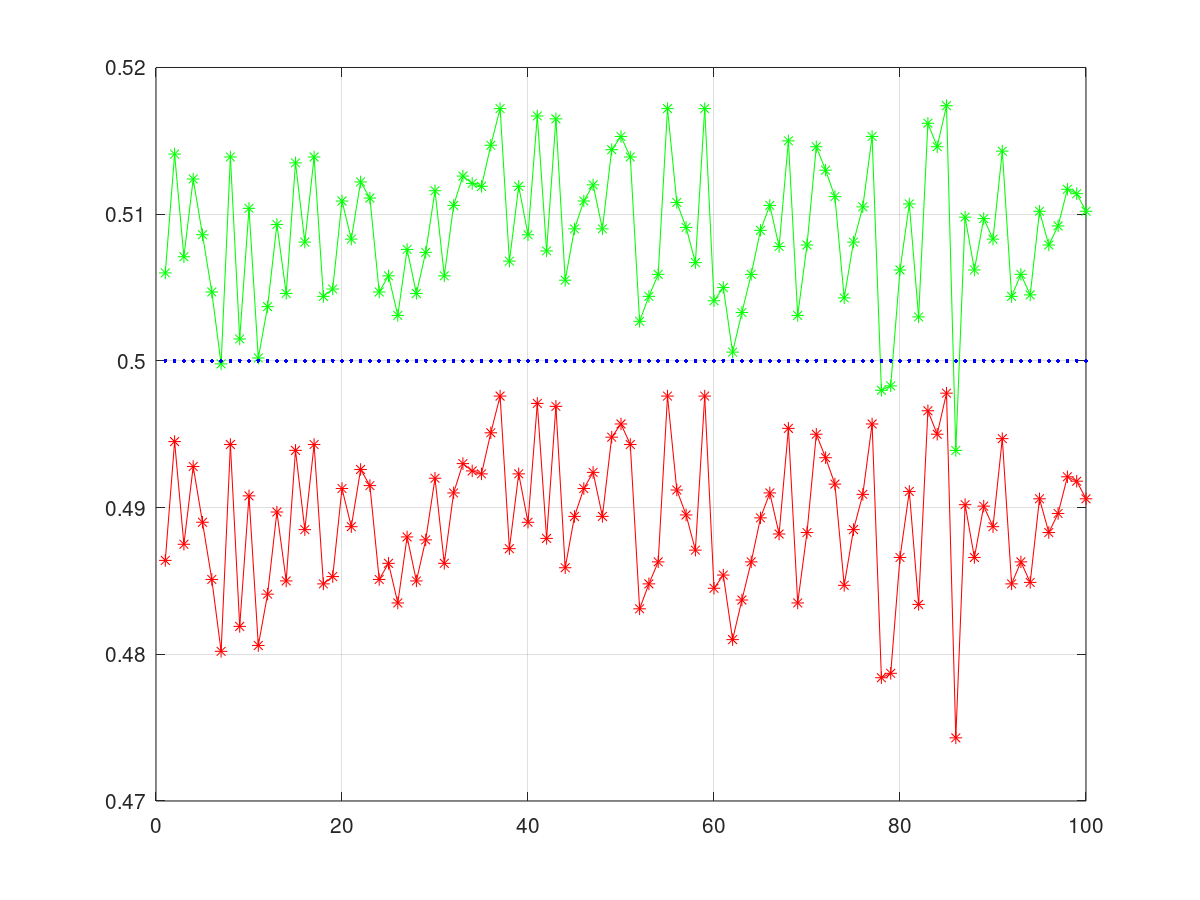
\includegraphics[width=1\linewidth]{diagram.png}}
    	    \end{figure}
            \begin{itemize}
                \item Зеленый~--- верхние границы доверительных интервалов,
                \item Синий~--- $P(X_i < t_0) = 0.5$,
                \item Красный~--- нижние границы доверительных интервалов.
            \end{itemize}
    \section{Вывод}
        Доля (96 из 100) доверительных интервалов, в которые попадает значение из генеральной совокупности, удовлетворяет оценке $\gamma$.
\end{document}
